\documentclass{article}\usepackage[]{graphicx}\usepackage[]{xcolor}
% maxwidth is the original width if it is less than linewidth
% otherwise use linewidth (to make sure the graphics do not exceed the margin)
\makeatletter
\def\maxwidth{ %
  \ifdim\Gin@nat@width>\linewidth
    \linewidth
  \else
    \Gin@nat@width
  \fi
}
\makeatother

\definecolor{fgcolor}{rgb}{0.345, 0.345, 0.345}
\newcommand{\hlnum}[1]{\textcolor[rgb]{0.686,0.059,0.569}{#1}}%
\newcommand{\hlsng}[1]{\textcolor[rgb]{0.192,0.494,0.8}{#1}}%
\newcommand{\hlcom}[1]{\textcolor[rgb]{0.678,0.584,0.686}{\textit{#1}}}%
\newcommand{\hlopt}[1]{\textcolor[rgb]{0,0,0}{#1}}%
\newcommand{\hldef}[1]{\textcolor[rgb]{0.345,0.345,0.345}{#1}}%
\newcommand{\hlkwa}[1]{\textcolor[rgb]{0.161,0.373,0.58}{\textbf{#1}}}%
\newcommand{\hlkwb}[1]{\textcolor[rgb]{0.69,0.353,0.396}{#1}}%
\newcommand{\hlkwc}[1]{\textcolor[rgb]{0.333,0.667,0.333}{#1}}%
\newcommand{\hlkwd}[1]{\textcolor[rgb]{0.737,0.353,0.396}{\textbf{#1}}}%
\let\hlipl\hlkwb

\usepackage{framed}
\makeatletter
\newenvironment{kframe}{%
 \def\at@end@of@kframe{}%
 \ifinner\ifhmode%
  \def\at@end@of@kframe{\end{minipage}}%
  \begin{minipage}{\columnwidth}%
 \fi\fi%
 \def\FrameCommand##1{\hskip\@totalleftmargin \hskip-\fboxsep
 \colorbox{shadecolor}{##1}\hskip-\fboxsep
     % There is no \\@totalrightmargin, so:
     \hskip-\linewidth \hskip-\@totalleftmargin \hskip\columnwidth}%
 \MakeFramed {\advance\hsize-\width
   \@totalleftmargin\z@ \linewidth\hsize
   \@setminipage}}%
 {\par\unskip\endMakeFramed%
 \at@end@of@kframe}
\makeatother

\definecolor{shadecolor}{rgb}{.97, .97, .97}
\definecolor{messagecolor}{rgb}{0, 0, 0}
\definecolor{warningcolor}{rgb}{1, 0, 1}
\definecolor{errorcolor}{rgb}{1, 0, 0}
\newenvironment{knitrout}{}{} % an empty environment to be redefined in TeX

\usepackage{alltt}
\usepackage{amsmath} %This allows me to use the align functionality.
                     %If you find yourself trying to replicate
                     %something you found online, ensure you're
                     %loading the necessary packages!
\usepackage{amsfonts}%Math font
\usepackage{graphicx}%For including graphics
\usepackage{hyperref}%For Hyperlinks
\usepackage[shortlabels]{enumitem}% For enumerated lists with labels specified
                                  % We had to run tlmgr_install("enumitem") in R
\hypersetup{colorlinks = true,citecolor=black} %set citations to have black (not green) color
\usepackage{natbib}        %For the bibliography
\setlength{\bibsep}{0pt plus 0.3ex}
\bibliographystyle{apalike}%For the bibliography
\usepackage[margin=0.50in]{geometry}
\usepackage{float}
\usepackage{multicol}

%fix for figures
\usepackage{caption}
\newenvironment{Figure}
  {\par\medskip\noindent\minipage{\linewidth}}
  {\endminipage\par\medskip}
\IfFileExists{upquote.sty}{\usepackage{upquote}}{}
\begin{document}

\vspace{-1in}
\title{Lab 05 -- MATH 240 -- Computational Statistics}

\author{
  Danny Molyneux \\
  Colgate University  \\
  Mathematics  \\
  {\tt dmolyneux@colgate.edu}
}

\date{Feb 10 2024}

\maketitle


\begin{multicols}{2}
\begin{abstract}
In this lab we are tasked with using \texttt{tidyverse} \citep{tidy} to gather stats for each musical feature for all three artists (The Front Bottoms, Manchester Orchestra, and All Get Out). We also extract these feature values for their combined song, Allentown. Then, use this information to answer the overarching question: Which band contributed most to the song Allentown?
\end{abstract}

\noindent \textbf{Keywords:} tidyverse; summarizing; analyzing; plotting
\section{Introduction}
The goal here is to address the question ``Which band contributed most to the song Allentown?". We have over 200 different features, for 181 different songs. The idea is to extract information on each band by looking at their batch of songs, and compare that information to the features of the song Allentown. Hopefully, we will see significant differences, and that one band has clearly more similar traits to that of Allentown. I will be sure to make various plots/graphs to get various insights and eventually come to a conclusion.
\section{Methods}
The data we are working with here is two .csv files, one with all of the features for Allentown, and one for the features for the other 180 \texttt{Essentia} \citep{Essentia} files. These features came from both \texttt{Essentia} and \texttt{LIWC} \citep{liwc}. Using \texttt(tidyverse), I use methods such as \texttt{group\textunderscore by()} and \texttt{summarize()} to create a data frame containing a multitude of statistics for each feature, grouped by artist. So this will look at each artist, take all of their songs from the csv file, and summarize the features. 

The \texttt{mutate()} function was very helpful as it allows me to create new columns that describe whether each artist is ``Out of Range", ``Outlying", or ``Within Range" for each feature.

The \texttt{xtable} library \citep{xtable} allows me to create a table that summarizes select features, so that we can pick and choose which features we want to use to answer the overarching question.

Lastly, using \texttt{ggplot} \citep{ggplot} is a way to really visualize our findings. Similarly to the \texttt{xtable}, we can plot specific features to see how the artists compare to Allentown's feature. Alternatively, we can use \texttt{ggplot} to compare the artists overall comparison's to Allentown, by calculating the proportion of each description (Out of Range, Outlying, Within Range) for each artist. I do this by creating a new data frame that for each artist, has both a count and proportion for each description type. We would plot this by putting the plot for each artist side-by-side.
\section{Results}
After collecting all of the data into my various data frames, here is the table I make for the four features that I especially wanted to analyze:
\begin{table}[H]
\centering
\begin{tabular}{rlll}
  \hline
 & artist & feature & description \\ 
  \hline
1 & All Get Out & overall\_loudness & Within Range \\ 
  2 & Manchester Orchestra & overall\_loudness & Within Range \\ 
  3 & The Front Bottoms & overall\_loudness & Outlying \\ 
  4 & All Get Out & danceability & Within Range \\ 
  5 & Manchester Orchestra & danceability & Within Range \\ 
  6 & The Front Bottoms & danceability & Out of Range \\ 
  7 & All Get Out & duration & Within Range \\ 
  8 & Manchester Orchestra & duration & Within Range \\ 
  9 & The Front Bottoms & duration & Within Range \\ 
  10 & All Get Out & emotion & Within Range \\ 
  11 & Manchester Orchestra & emotion & Within Range \\ 
  12 & The Front Bottoms & emotion & Within Range \\ 
   \hline
\end{tabular}
\caption{Results of each essentia feature vs Allentown} 
\label{range_results:reference}
\end{table}
So although I liked the idea of using emotion and duration, they ended up not being very helpful, because each artist is within range for those features, meaning the Allentown feature is within their lower fence ($Q1 - 1.5IQR$) and upper fence ($Q3 + 1.5IQR$). So these two features don't seem to give us much insight at all. However, if you look at the box plot below, you will see that Allentown's duration is quite a bit further away from Manchester Orchestra's median than the others. This still doesn't tell us much, because it's one feature and they are all still relatively close to the median. \\

On the other hand, we learn a lot from the table and box plot about overall loudness and danceability. Allentown is Out of Range and Outlying in regards to The Front Bottoms' danceability and overall loudness, respectively. For the other two bands, both features are within range. So if you find these two traits valuable, it may lead you to believe that The Front Bottoms weren't as contributive to Allentown as Manchester Orchestra and All Get Out.
\begin{knitrout}\scriptsize
\definecolor{shadecolor}{rgb}{0.969, 0.969, 0.969}\color{fgcolor}
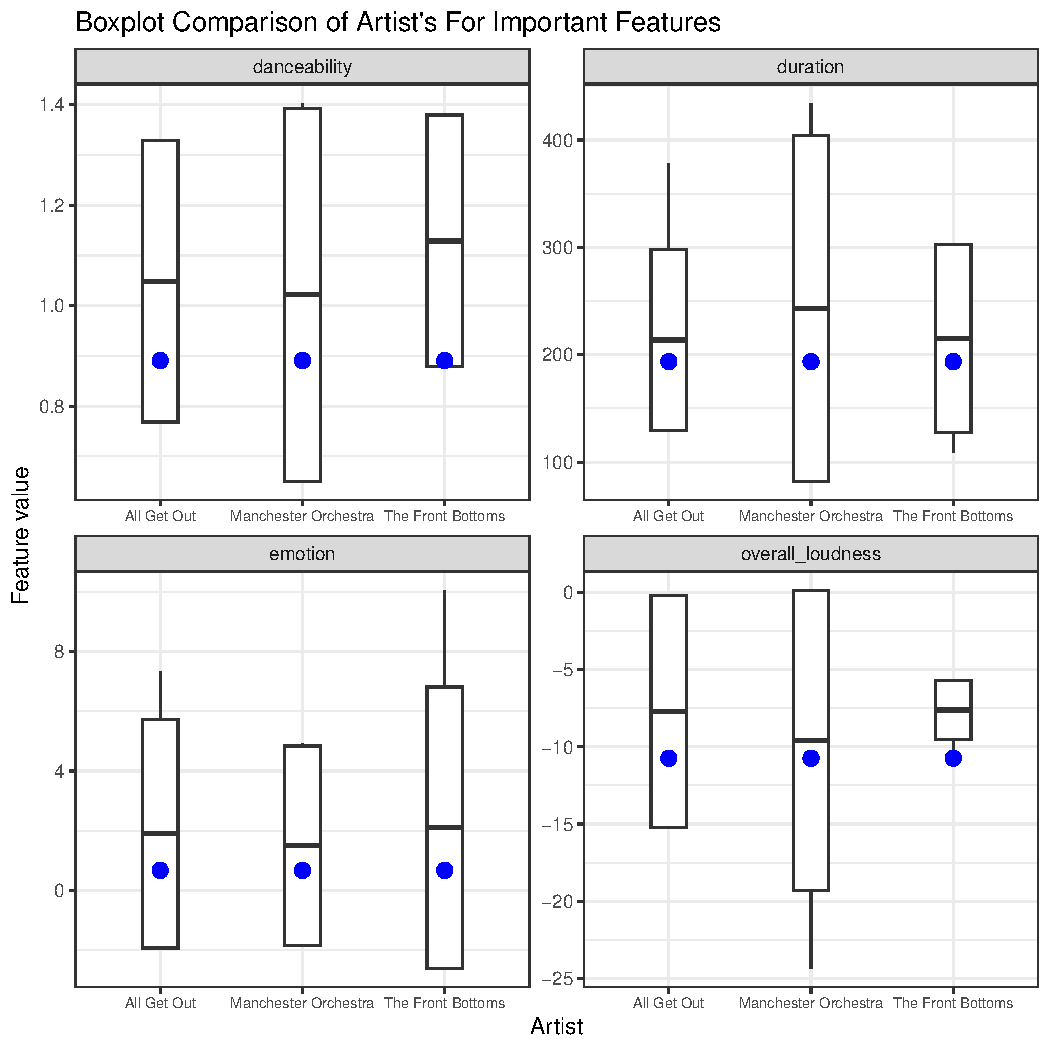
\includegraphics[width=\maxwidth]{figure/unnamed-chunk-1-1} 
\end{knitrout}
As I mentioned in the Methods section, I also use ggplot to analyze the artists as a whole, rather than for specific features. To do so, I made a few different side-by-side plots, comparing the proportions of descriptions for each artist. Let's start by looking at the pie chart and doughnut plot I have made, because they are quite similar graph types.
\begin{knitrout}\scriptsize
\definecolor{shadecolor}{rgb}{0.969, 0.969, 0.969}\color{fgcolor}
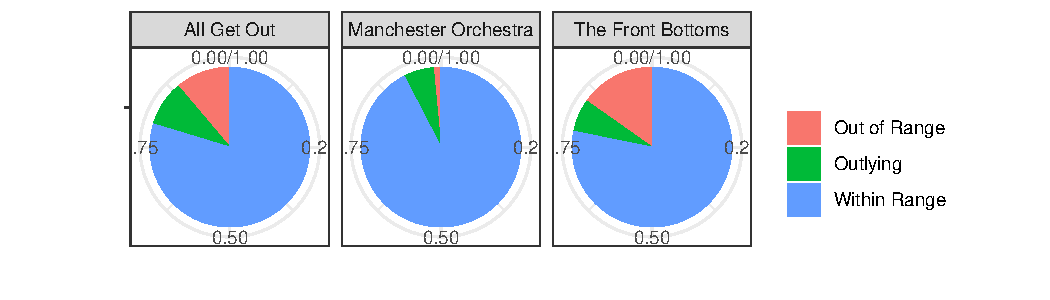
\includegraphics[width=\maxwidth]{figure/unnamed-chunk-2-1} 

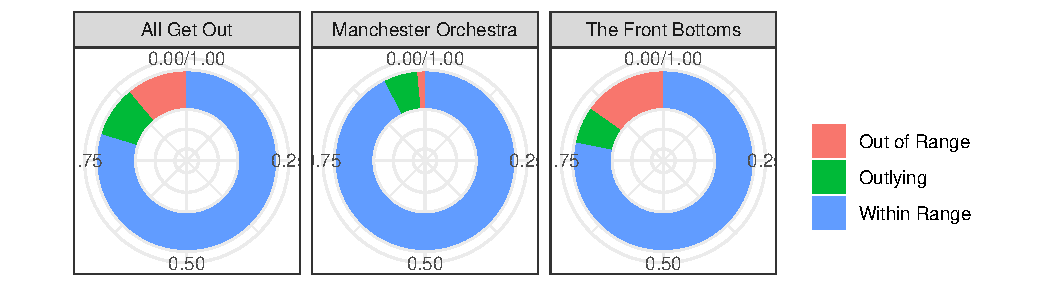
\includegraphics[width=\maxwidth]{figure/unnamed-chunk-2-2} 
\end{knitrout}
I really like these plots (doughnut more than pie) because they tell you in general, which bands were more often in the same range as Allentown, as well as the contrary. I think these plots are very much so in favor of Manchester Orchestra being the band that contributed most to Allentown. They have the highest proportion of ``Within Range" and the lowest proportion of ``Out of Range". In regards to the other two bands, it isn't super obvious, but All Get Out has a slightly higher proportion of `Within Range" and definitely has a smaller proportion of ``Out of Range". Also note that I am using proportions rather than just counting, because the sample size for each band is different. Let's look at one more plot in case the doughnut/pie plots were too difficult to visualize. Here is a column plot of the same data:
\begin{knitrout}\scriptsize
\definecolor{shadecolor}{rgb}{0.969, 0.969, 0.969}\color{fgcolor}
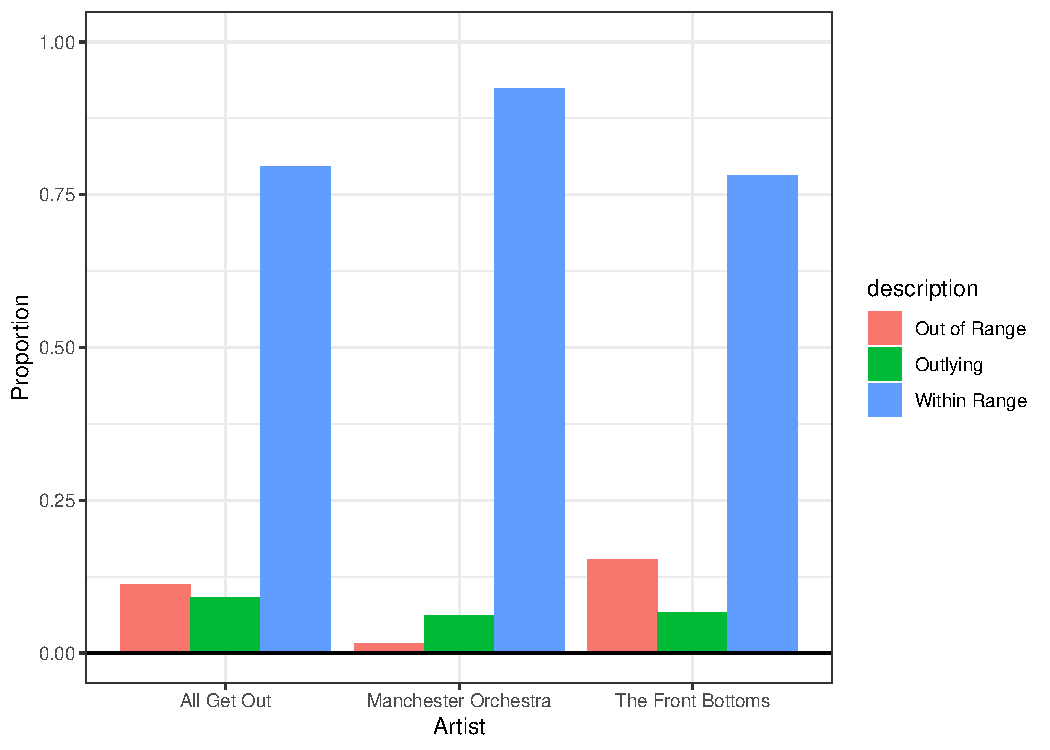
\includegraphics[width=\maxwidth]{figure/unnamed-chunk-3-1} 
\end{knitrout}
This tells the same story, but maybe a little more clearly.
\section{Discussion}
So those last three graphs definitely gave us some strong leads to answer this question, but is it conclusive? I'd say no. The reason is, we don't know exactly which features fall under which description for each artist. And how do we weigh each feature? I know I chose those four features earlier that I thought were especially important, but I am by no means a musical expert. For all we know, the four most significant features were within range for The Front Bottoms, and Out of Range for the other two bands. Is it likely? No. But it is possible.\\
The othr thing we must keep in mind is that even if Allentown is more similar to the sample of The Front Bottoms songs we have, doesn't mean they actually contributed more. If we kept increasing the sample size, we could probably say it with high confidence, but Allentown could always be an outlier. So how could we answer this question with more certainty other than increasing sample size?
\begin{tiny}
\bibliography{bibliography}
\end{tiny}
\end{multicols}




\end{document}

